
\chapter{Introduction}

This chapter begins by explaining the motivation for the work
described in this dissertation.
Afterwards, the objectives of the work, which come from the
motivation, are described and then the approach taken in the work is
discussed. 
Finally, the structure of the remainder of this dissertation is
described.

\section{Motivation}

Since its release in 1995, the Java programming
language~\cite{gosling2013} has increased in popularity and is now in
use on many platforms.
This popularity means that Java has been used in a wide variety of
areas including desktop applications, on the internet in the form of
Java applets, on smartcards~\cite{chen2000} and on mobile
devices~\cite{oracle2014}.
Several languages derived from Java have also been created, including
Scala~\cite{lausanne2015} and Ceylon~\cite{redhat2015}, as well as
older variants of Java such as MultiJava~\cite{clifton2006} and
Pizza~\cite{odersky1997}, which have in turn contributed to the
development of Java.
Scala adds functional programming features to Java, some of which have
been incorporated into Java 8.
Ceylon extends Java's type system with features such as union types,
allowing some common Java errors to be checked at compile time through
the type system.

One use of Java that is of particular interest is in embedded systems.
While early versions of Java were developed for programming embedded
systems, particularly TV set-top boxes, the technology was not well
received.
It was only in the growing sector of the internet that Java initially
found a market~\cite{horstmann2002}.
However, it was soon realised that the portability, modularity, safety
and security benefits of Java could be of great use in embedded
systems~\cite{mulchandani1998}.
This required the creation of specialised Java virtual machines as the
standard JVM is too large for most embedded systems.
Much research has gone into making smaller and smaller virtual
machines to widen the range of devices that Java can be used
on~\cite{caska2011,thomm2010}.

Many embedded systems are also real-time systems, and features of Java
such as the garbage collector and the concurrency model make it
unsuitable for real-time systems, for which strict guarantees about
timing properties must be made.
To address this issue the Real-Time Specification for Java
(RTSJ)~\cite{gosling2000} was created.
The RTSJ extends Java with a scoped memory model and a more
predictable scheduling system.

While the RTSJ addresses real-time requirements of embedded systems,
many embedded systems are also safety-critical.
For these conformance to certain standards, such as \mbox{DO-178C} and
ISO~26262, is required.
To support the development of safety-critical programs that meet these
requirements in Java, the Safety-Critical Java (SCJ)
specification~\cite{locke2013} has been created.
SCJ is a subset of the RTSJ that removes the features that cannot be
easily statically reasoned about, which means that features such as
the garbage-collected heap and dynamic class loading are absent from
SCJ.
This facilitates the creation of SCJ programs that fulfil formal
specifications; indeed work has already been done on developing
correct SCJ programs from formal specifications~\cite{cavalcanti2011,
  cavalcanti2013}.

On the other hand, even if it can be shown that SCJ programs are
correct, it must still be ensured those programs are executed
correctly.
In the case of Java-like languages, this generally means ensuring the
Java compiler and Java Virtual Machine (JVM) are correct.

Work has been done on modelling virtual machines for Java, and on the
formal correctness of compilers targeting those virtual machines.
Some of the most complete work in that area was by St\"{a}rk, Schmid
and B\"{o}rger~\cite{stark2001}, who present a model of the full Java
language and virtual machine, along with a formally verified compiler,
although for an older version of Java than is current.
Other work has also been done on modelling the JVM and Java
compilation using refinement techniques~\cite{duran2010}.
Additionally there has been work considering machine checked models of
Java virtual machines and compilers~\cite{lochbihler2012, nipkow2000,
  strecker2002}.
Work has also been done on the semantics of Java bytecode and
verification of standard JVMs~\cite{bertelsen2000, jones1998}.

However, SCJ has a number of differences from standard Java.
Firstly, as already indicated the SCJ memory model is rather different
to the standard Java memory model, abandoning the garbage collector in
favour of a scoped memory model.
Garbage collection is less predictable and often quite complex, and so
difficult to reason about and unsuitable for some of the strictest
certifiability requirements of safety-critical systems.
By contrast, the scoped memory model provides greater predictability
on when memory is freed.
Similarly, the SCJ approach to scheduling differs from that of
standard Java, using a preemptive priority scheduling approach rather
than the unpredictable scheduling of standard Java threads.
These differences of SCJ from standard Java mean that the standard JVM
is not suitable for running SCJ programs.
A specialised virtual machine is required.

In the case of virtual machines for embedded systems, the priorities
are usually size and speed, which generally results in machines that
are hard to verify.
Moreover, virtual machines that rely on interpreting bytecode are
unsuitable for real-time embedded systems as they are likely to be
slower.
An alternative method to run a Java program is to compile it to native
code and some authors have suggested doing so either
directly~\cite{schultz2003} or via C~\cite{varma2004}.
There are several virtual machines that take this approach including
Fiji VM~\cite{pizlo2009}, Icecap HVM~\cite{sondergaard2012} and
OVM~\cite{armbruster2007}.
This allows correct running of an otherwise correct SCJ program to be
viewed as a compiler verification problem.

There has been much research into compiler correctness.
Much of the work follows a commuting diagram approach, in which the
compilation is shown to be consistent with transformation between the
semantics of the source and target languages\cite{morris1973,
  thatcher1979}.
This approach is apparent in much of the early work such as that of
McCarthy and Painter~\cite{mccarthy1967}, as well as in more recent
work such as the CompCert project~\cite{leroy2009a, leroy2009b}.
There has also been work that follows this approach and employs
automated theorem provers~\cite{klein2006, milner1972, nipkow2000}.
They provide additional certainty that the proof is correct and can
also provide code generation facilities to allow creation of a working
compiler.

An alternative is the algebraic approach to compiler
verification~\cite{hoare1991, sampaio1993}, based on modelling
compilation using refinement calculi~\cite{back1981, morgan1990,
  morris1987}.
This approach appears to be less commonly used but has been applied to
Java~\cite{duran2005, duran2010} and hardware description
languages~\cite{perna2010, perna2011}.
This approach is also quite amenable to automation as it relies on
refinement laws that can be applied by a term rewriting system.

There is a clear need for formal verification of SCJ virtual machines
due to the safety-critical nature of the systems involved and the fact
that safety standards such as DO-178C require it at the highest safety
levels.
However, there appears to be little work done in that area and, as far
as we know, no SCJ virtual machine has been formally verified.

% explain that there is a gap with no verification for SCJ compilers
% for embedded systems

\section{Objectives}

Our objective is to develop an approach to verification of an SCJ
virtual machine that allows the production and verification of correct
SCJ virtual machines.
Although the actual creation and verification of such machines is
outside the scope of our work, we provide the following resources for
developers and verifiers:
\begin{itemize}
\item a specification of the requirements of an SCJ virtual machine,
\item a formal model of the virtual machine specification,
\item a compilation strategy from Java bytecode to native C code,
\item proofs for validation of the formal model and verification of
  the compilation strategy, and
\item a mechanisation of the model and proofs.
\end{itemize}

We follow the design of existing SCJ virtual machines to ensure that
our work is of practical relevance to the SCJ community.
We particularly focus on the icecap HVM~\cite{sondergaard2012}, as
that is the only publicly-available SCJ virtual machine that is
up-to-date with the SCJ specification.
Where there are ambiguities or concerns regarding the description of
the virtual machine in the SCJ standard, we take the icecap
implementation as a reference to define the requirements and formal
model for an SCJ virtual machine.
In addition, the native C code generated by our formal compilation
strategy is very close
% TODO: check this near the end of the work when we know what is
% achieved
to that actually produced by icecap.
%This is an assurance of the practical relevance of our results.

Our results can be used to aid the development and verification of an
SCJ virtual machine in several different ways.
The informal specification provides a reference for the requirements
of an SCJ virtual machine, while the formal model can be used to prove
correctness of an implementation.
The formal model could also be used to create a
correct-by-construction virtual machine via refinement steps.
Similarly, the specification of the compilation strategy can be used
to translate SCJ bytecode to equivalent C code, which may be used to
add compilation facilities to an SCJVM.
The proofs give further assurance of the correctness of the model and
compilation strategy.
Additionally, the mechanisation can better facilitate the use of the
other components of the work.


\subsection{SCJ Virtual Machine Specification}

The first component required is a specification of the requirements
for an SCJ virtual machine.
This specification will shape the rest of the work and there is at
present no clear specification of what is required of an SCJ virtual
machine or how it differs from a standard Java virtual machine.
The specification of requirements needs to consider the requirements
imposed, both explicitly and implicitly, on virtual machines by the
SCJ specification~\cite{locke2013} as that provides the authoritative
source for information on SCJ.
It is also helpful to consider the approach taken by some existing SCJ
virtual machines on points where the SCJ specification is unclear.
The virtual machine must also meet the standard Java Virtual Machine
specification~\cite{lindholm2014} on points such as how to interpret
Java bytecode instructions.
There is much existing work on the semantics of Java bytecode that can
be used in our work~\cite{bertelsen2000, jones1998, stark2001}.

\subsection{Compilation Strategy}

As many existing virtual machines for SCJ precompile programs to
native code in order to allow faster execution on embedded systems, it
seems wise to include that in our approach.
We will focus on compilation of Java bytecode to C as that is the
approach adopted by several existing virtual machines for embedded
systems, including Fiji VM~\cite{pizlo2009} and icecap
HVM~\cite{sondergaard2012}, and C is already widely used for embedded
systems software.

There are two main approaches to the specification and verification of
compilers: the commuting diagram approach and the algebraic approach.
The commuting diagram approach involves specifying the compiler as a
function from the source language to the target language and showing
that it is consistent with transformation between the semantics of the
source and target languages~\cite{morris1973, thatcher1979}.
This approach has been used in much of the work on compiler
correctness, including some of the earliest work~\cite{mccarthy1967}
and recent work such as that of the CompCert project~\cite{leroy2009a,
  leroy2009b}.

The algebraic approach involves defining the source and target
languages in the same specification space, and using proved
specialised rewrite rules to characterise compilation as model
transformation in the extended language.
This approach was first proposed in the early nineties by
Hoare~\cite{hoare1991} and further developed by
Sampaio~\cite{hoare1993, sampaio1993}.
The algebraic approach does not seem to be as popular as the commuting
diagram approach, but it does have the advantage that the
specification of the compilation strategy is correct by construction
as the rewrite rules that comprise it have all been proved.

We adopt the algebraic approach in our work, since it does not require
the additional function that is required in the commuting-diagram
approach because the source and target languages are defined in terms
of the same specification language.
The algebraic approach also permits a modular approach to proof and
allows for the compiler to be easily implemented by application of the
refinement rules using a term rewriting system.
This means we can more easily evaluate the compilation strategy.

\subsection{Formal Model and Proofs}

As we are following the algebraic approach, we require a specification
language in which to define the source and target languages.
The use of a formal specification language for our specification of an
SCJVM allows us to ensure that the specification is precise and to
facilitate proofs of its correctness.
This is beneficial for both the parts of the SCJVM that are involved
in the compilation and the parts are not.

We have chosen \Circus{} as the specification
language~\cite{oliveira2009} as it contains a wide variety of
constructs that allow for specification of both data and behaviour,
with a inbuilt notion of refinement, which we require for specifying
the compilation strategy.
\Circus{} has also been used for previous work on the specification of
SCJ programs~\cite{cavalcanti2011, cavalcanti2013}.

It is important that the correctness of the formal models and
compilation strategy can be shown via mathematical proof, which
requires the specification language to have a well-defined semantics.
\Circus{} has such a semantics, defined using the model of Unifying
Theories of Programming (UTP)~\cite{hoare1998}.

\subsection{Mechanisation}

To prevent mistakes in the proofs, it is helpful to mechanise the
formal model and proofs.
There are various systems that can be used for this, but we will focus
on the proof assistant Isabelle~\cite{nipkow2002, nipkow2014}.
It has existing mechanisations of \Circus{}~\cite{feliachi2012} and
the UTP~\cite{foster2015}, and has been used in previous work
verifying compilers for Java-like languages~\cite{klein2006,
  strecker2002, lochbihler2010}, making it well placed for our work.

\subsection{Summary}

In conclusion, our objective is an approach verification of SCJVMs
consisting of mechanised formal models together with proofs of
properties about them.
These formal models will cover both the services that must be provided
by a running SCJVM and a compilation strategy for translating Java
bytecode to native code.
With our results, SCJVM developers will be able to create provably
correct ahead-of-time compiling SCJVM implementations and check the
correctness of those implementations.

\section{Approach}

As mentioned above, we follow the algebraic approach to verifying
compilation, refining our model of Java bytecode to a representation
of C code.
The standard algebraic approach, developed by Hoare and Sampaio,
follows the form shown in Figure~\ref{algebraic-approach-figure}.
The source program is defined by a shallow embedding in the
specification language and this is then refined to a model of the
target machine in the specification language that contains the target
code for the program.

\begin{figure}
  \centering
  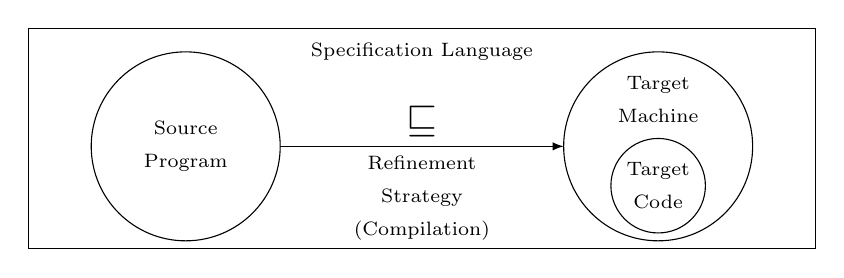
\begin{tikzpicture}
    \draw (0cm,0.7cm) rectangle (10cm,3.5cm);
    \draw (5cm,3.2cm) node[align=center] {\scriptsize Specification Language};

    \draw (2cm,2cm)   circle[radius=1.2cm]               node[align=center] {\scriptsize Source\\\scriptsize Program};
    \draw (8cm,2cm)   circle[radius=1.2cm] ++(0cm,0.6cm) node[align=center] {\scriptsize Target\\\scriptsize Machine};
    \draw (8cm,1.5cm) circle[radius=0.6]                 node[align=center] {\scriptsize Target\\\scriptsize Code};

    \path (3.2cm,2cm) edge[-latex]
    node[align=center, above] {\Large $\sqsubseteq$}
    node[align=center, below] {\scriptsize Refinement\\\scriptsize Strategy\\\scriptsize (Compilation)}
    (6.8cm,2cm);
  \end{tikzpicture}
  \caption{Standard algebraic approach}
  \label{algebraic-approach-figure}
\end{figure}

The standard algebraic approach is normally applied to compile from a
high-level language to a low-level language executable in a target
machine.
Here, we adapt the approach to deal with a low-level source language,
Java bytecode.
While Java bytecode has some high-level features, particularly its
notion of objects, we view it as low-level since it is unstructured,
with control flow managed using a program counter.

Our approach can be viewed as the usual approach applied in reverse,
starting with an interpreter containing the bytecode source program,
and proving that it is refined by an embedding of the C code, as shown
in Figure~\ref{our-approach-figure}.
The core services of an SCJVM, such as scheduling and memory
management, must be available for both the source and target codes.

For a low-level language, a deep embedding is the
natural method for representing its semantics, since it is defined in
terms of how it is processed by a (virtual) machine.
For the C code we must choose whether to use a shallow embedding,
representing C constructs by corresponding \Circus{} constructs, or a
deep embedding, creating a \Circus{} model that interprets the C
code.

\begin{figure}
  \centering
  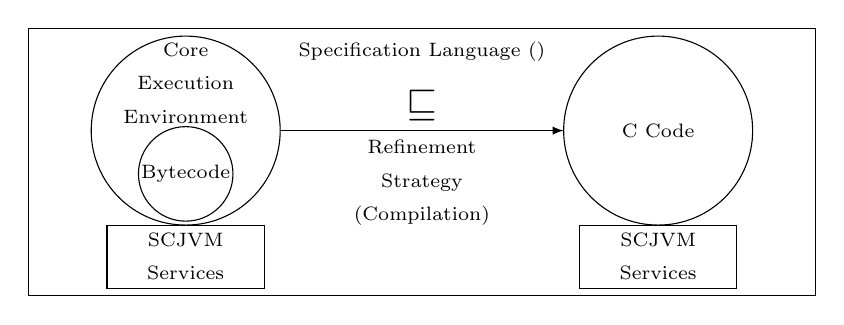
\begin{tikzpicture}
    \draw (0cm,0.4cm) rectangle (10cm,3.8cm);
    \draw (5cm,3.5cm) node[align=center] {\scriptsize Specification Language (\Circus{})};

    \draw (2cm,2.5cm)   circle[radius=1.2cm] ++(0cm,0.6cm) node[align=center] {\scriptsize Core\\\scriptsize Execution\\\scriptsize Environment};
    \draw (2cm,1.95cm)     circle[radius=0.6cm]               node[align=center] {\scriptsize Bytecode};
    \draw (8cm,2.5cm)   circle[radius=1.2cm]               node[align=center] {\scriptsize C Code};

    \draw (1cm,0.5cm) rectangle (3cm,1.3cm) node[pos=0.5,align=center] {\scriptsize SCJVM \\\scriptsize Services};
    \draw (7cm,0.5cm) rectangle (9cm,1.3cm) node[pos=0.5,align=center] {\scriptsize SCJVM \\\scriptsize Services};

    \path (3.2cm,2.5cm) edge[-latex]
    node[align=center, above] {\Large $\sqsubseteq$}
    node[align=center, below] {\scriptsize Refinement\\\scriptsize Strategy\\\scriptsize (Compilation)}
    (6.8cm,2.5cm);

    % \draw[-latex] (3cm,0.9cm) -- (7cm,0.9cm);
  \end{tikzpicture}
  \caption{Our algebraic approach}
  \label{our-approach-figure}
\end{figure}

We use a shallow embedding, since it allows existing algebraic laws
for \Circus{} to be used directly for manipulation of the C code
and proof of the compilation rules.
A deep embedding would require representing the syntax of C separately
in \Circus{} and rules for transforming the C code would have to be
proved.

The shallow embedding approach is much easier to extend or adapt. 
If a larger subset of bytecodes needs to be considered or the target C
code needs to be modified, in the worst case, we need more or
different \Circus{} compilation rules. 
There will be no need to extend the \Circus{} model defining the C
semantics. 

\section{Document Structure}

Having given a brief overview of the area of study and identified the
problem we wish to consider, the remainder of this dissertation
proceeds as follows.

In Chapter~\ref{literature-review-chapter} we examine the literature
on safety-critical virtual machines and compilers for Java-like
languages.
This includes a discussion of why a safety-critical variant of Java is
necessary and how it differs from standard Java.
We also explain why a specialised virtual machine is necessary for
SCJ.
This is followed by a survey of the existing virtual machines for
Safety-Critical Java and the techniques used in verifying compilers.

In Chapter~\ref{scjvm-services-chapter} we present an identification of the
requirements of SCJ virtual machine services, with a formal model of
those requirements in the \Circus{} specification language.
This is followed by a model of the an SCJ virtual machine core
execution environment in Chapter~\ref{cee-chapter}.

Finally, we conclude in Chapter~\ref{conclusions-chapter} by
summarising our contributions and mentioning the wider context of this
research.